\section{पीसीबी व एन्क्लोज़र}

	\subsection{पीसीबी}	
	
		\begin{figure}[ht!]
			\centering
			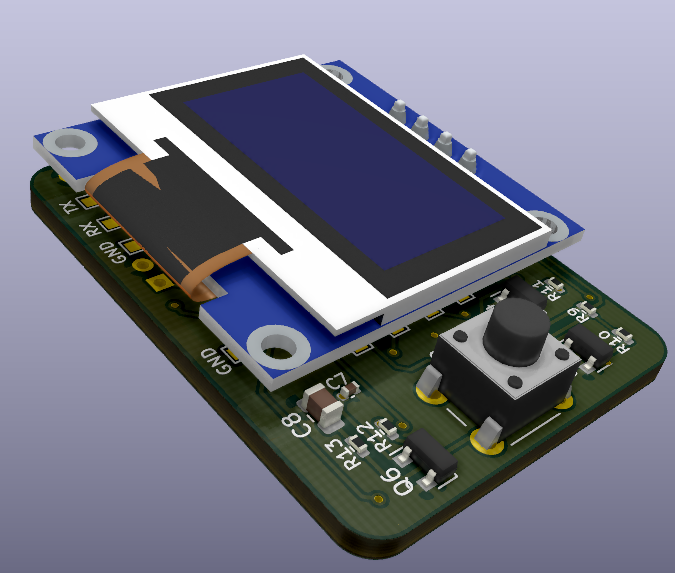
\includegraphics[width=0.6\textwidth]{../common/pcb/pcb.png}
			\caption{पूर्ण पीसीबी}
		\end{figure}


		\begin{figure}[ht!]
			\centering
			\subfloat[पीसीबी पिछ्ला भाग
			]{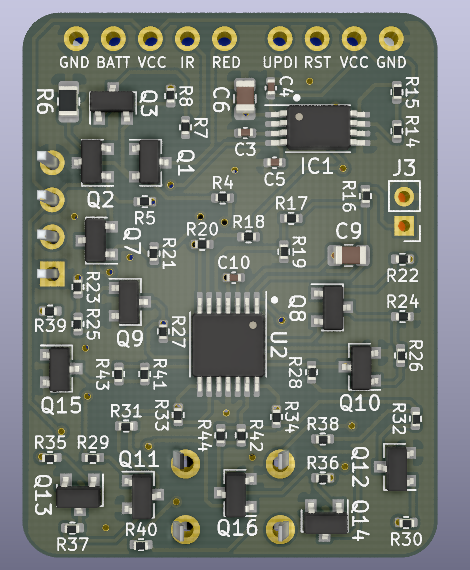
\includegraphics[width=0.5\textwidth]{../common/pcb/pcb_back.png}}
			\hfill
			\subfloat[पीसीबी अग्र भाग
			]{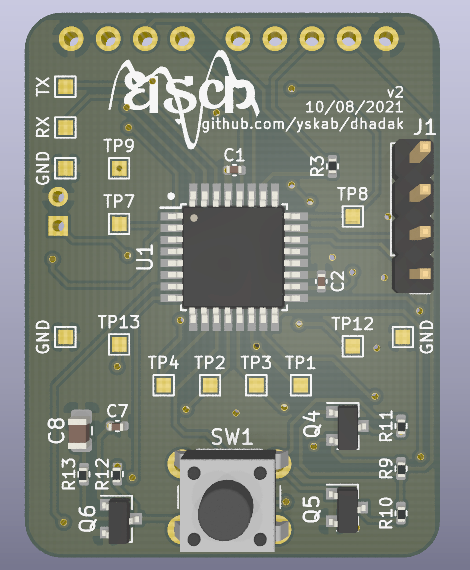
\includegraphics[width=0.5\textwidth]{../common/pcb/pcb_front.png}}
			\caption{पीसीबी के चित्र}
		\end{figure}

		पीसीबी डिजाइन को 2 परतों पर पूरा किया गया था जिसमें अधिकांश अंशो को पीछे की तरफ रखा गया था ताकि उन्हें डोसा पैन पर आसानी से री-फ़्लो किया जा सके। सामने की तरफ के सभी अंशो को हाथ से सोल्डर किया जाना है। 

		\begin{itemize}
			
			\item डिवाइस को संचालित करने के लिए एक सॉफ्ट लैच पावर ऑन/ऑफ स्विच सर्किट भी शामिल है।
			
			\item UPDI इंटरफ़ेस के माध्यम से $\mu$C को प्रोग्राम करने के लिए एक प्रोग्रामिंग हेडर भी लगाया गया था।
			
			\item Led, बैटरी और फोटोडायोड को जोड़ने के लिए कनेक्शन हेडर बनाये गए है जो एन्क्लोज़र के निचले हिस्से पर मौजूद होंगे।
			
			\item OLED डिस्प्ले के लिये हैडर। 

		\end{itemize}
	
		जांच के लिए आसान पहुंच और ऑसिलोस्कोप पर संकेतों को देखने के लिए सामने की तरफ पर्याप्त परीक्षण बिंदु जोड़े गए थे।
		
		पीसीबी साइज को OLED डिस्प्ले मॉड्यूल के बराबर रखने के लिए 0402 साइज रेसिस्टर्स/कैपेसिटर का इस्तेमाल किया गया।
					

	\subsection{एन्क्लोज़र}		
		
		एन्क्लोज़र को एक सरल ऑक्सीमीटर से संदर्भ लेते हुए डिज़ाइन किया गया था जिसमें शीर्ष पर डिस्प्ले \& PCB, निचला भाग पर फिंगर इंसर्ट और बैटरी कंपार्टमेंट है।
		
		\begin{figure}[ht!]
			\centering
			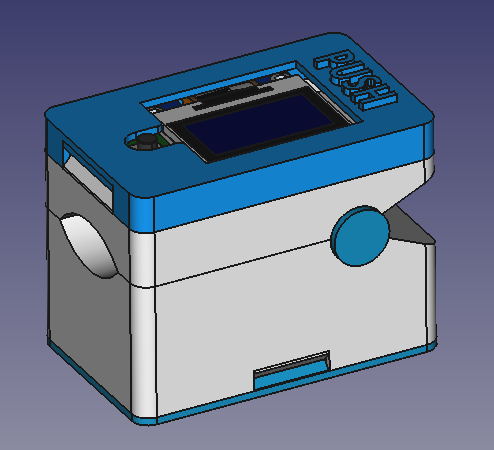
\includegraphics[width=0.5\textwidth]{../common/enc/enc.png}
			\caption{पूर्ण एन्क्लोज़र}
		\end{figure}	
				
		उपरि भाग पर फोटोडायोड और निचले में led एक चिंतनशील सेट अप मे मौजूद है। 
				
		\begin{figure}[ht!]
			\centering
			\subfloat[फोटोडायोड कम्पार्टमेंट
			]{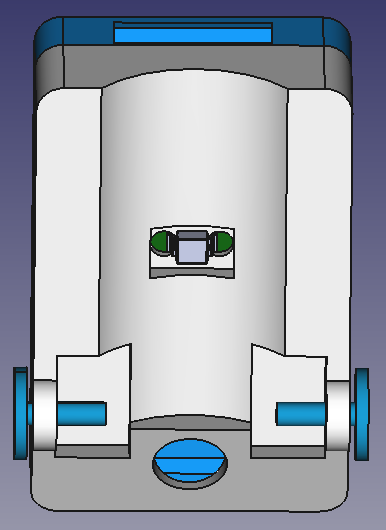
\includegraphics[width=0.45\textwidth]{../common/enc/top_base.png}}
			\hfill
			\subfloat[पीसीबी के लिए स्पेसर
			]{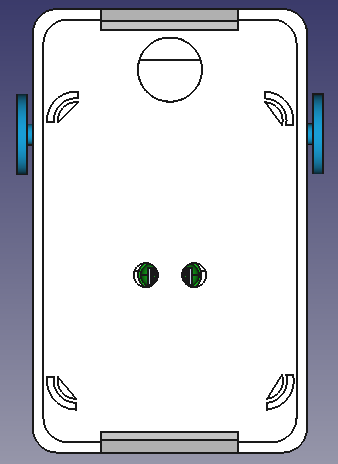
\includegraphics[width=0.45\textwidth]{../common/enc/top_base2.png}}
			\caption{उपरि भाग}
		\end{figure}
	
	
		\begin{figure}[ht!]
			\centering
			\subfloat[बैटरी कम्पार्टमेंट
			]{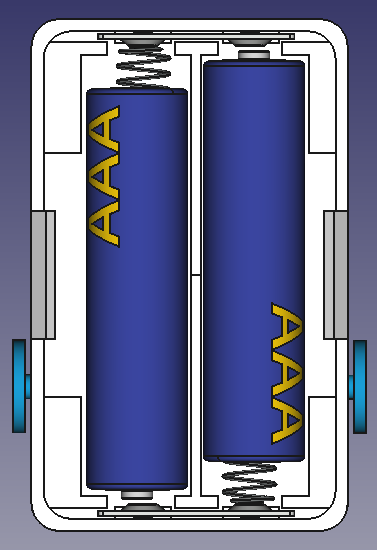
\includegraphics[width=0.45\textwidth]{../common/enc/bot_base.png}}
			\hfill
			\subfloat[Led कम्पार्टमेंट
			]{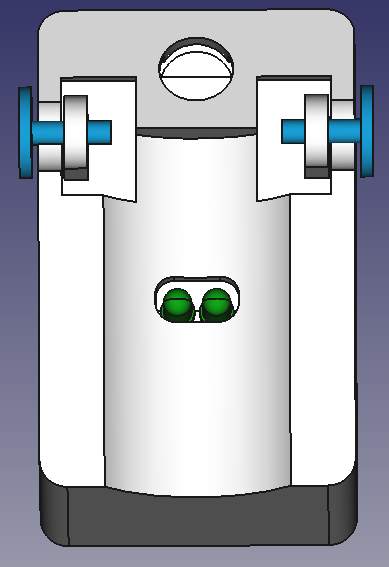
\includegraphics[width=0.45\textwidth]{../common/enc/bot_base2.png}}
			\caption{निचला भाग}
		\end{figure}
	
		उंगली को सुरक्षित करना एक महत्वपूर्ण हिस्सा है क्योंकि किसी भी तरह के डगमगाने या अनुचित संपर्क से सिग्नल की गुणवत्ता और गणना किए गए मापदंडों में गिरावट आ सकती है। उंगली पर एक मजबूत दबाव प्राप्त करना जरुरी है जो इसे स्थिर रखेगा, इसीलिये रोटेशन तंत्र में एक सेफ्टीपिन (क्लिप भाग को हटाकर) का उपयोग किया गया है।
		
		\begin{figure}[ht!]
			\centering
			\subfloat[सेफ्टीपिन
			]{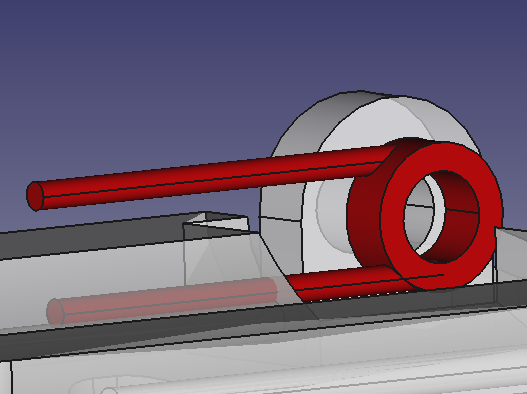
\includegraphics[width=0.5\textwidth]{../common/enc/pin.png}}
			\hfill
			\subfloat[सेफ्टीपिन का द्र्शय
			]{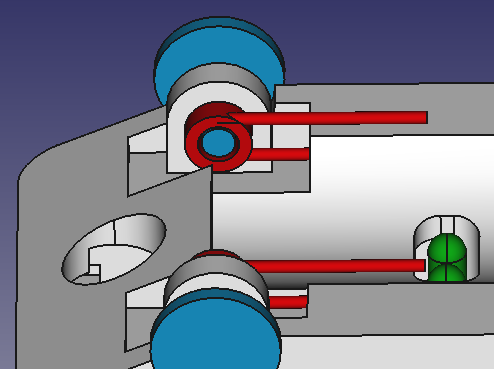
\includegraphics[width=0.5\textwidth]{../common/enc/pin_side.png}}
			\caption{सेफ्टीपिन निचले भाग मे}
		\end{figure}	
		
		निष्क्रिय स्थिति में, सेफ्टीपिन (पिन) प्राकृतिक गैर-विस्तारित अवस्था में होगा इसलिए दोनों  भाग बंद हो जाएंगे। जब उंगली डाली जायेगी, उपरि हिस्से को उठना होगा रोटेशन तंत्र के माध्यम से जभी उंगली अंदर जाएगी। इस से पिन उपरी भाग को उंगली पर नीचे धकेलेगा जिससे फोटोडायोड के साथ अच्छा संपर्क सुनिश्चित होगा और एक मजबूत पकड़ बनेगी। 

		\begin{figure}[ht!]
			\centering
			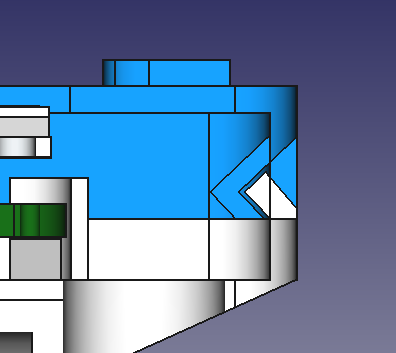
\includegraphics[width=0.6\textwidth]{../common/enc/snap.png}
			\caption{स्नैप फिट क्रॉस-सेक्शन}
		\end{figure}	
		
	
		स्नैप फिट तत्वों को लागू किया गया है जिससे जब भी आवश्यक हो कवर भागों को फिट करना और निकालना आसान हो सके। 